\section{AGI Autonomy with Hard Safety Boundaries}\label{sec:autonomy}

Autonomous AI in financial markets raises a fundamental tension: the system must be free to experiment, learn, and adapt, yet every autonomous action affects real capital. PolyEdge addresses this tension through a four-boundary safety framework (ADR-006) that enforces hard, deterministic constraints on autonomous behavior. These boundaries are non-bypassable: no agent, human or artificial, can override them without changing the underlying configuration \citep{amodei2016concrete, russell2020human}.

\subsection{Four Hard Boundaries}

\subsubsection{Boundary 1: Strategy Composition Bounded by Risk Profiles}

Every strategy, whether human-authored or AI-generated, must validate through the \texttt{RiskManager} pipeline before any capital is deployed. The risk profiles defined in ADR-005 (safe, normal, aggressive, extreme) establish non-bypassable limits on position size (as a fraction of bankroll), maximum drawdown, daily loss limits, and portfolio concentration. An AI-generated strategy that proposes a position exceeding the active profile's \texttt{MAX\_POSITION\_FRACTION} is automatically rejected; the rejection reason is logged in the \texttt{TradeAttempt} ledger for post-hoc analysis. This boundary ensures that creative exploration by the autonomy system cannot violate the capital-protection mandates.

\subsubsection{Boundary 2: Deterministic Promotion Pipeline}

Autonomously generated strategy code follows a strict validation pipeline before it can access real capital. The pipeline has six stages:

\begin{enumerate}
    \item \textbf{DRAFT.} Code is generated (by LLM or human) but is not executed. It resides in isolated experiment state.
    \item \textbf{BACKTEST.} The strategy is validated against historical market data. The backtest computes Sharpe ratio, win rate, and maximum drawdown. If performance falls below thresholds, the strategy is retired after a 7-day grace period.
    \item \textbf{SHADOW.} The strategy runs in paper-trading mode with a simulated bankroll. It generates signals, passes through risk validation, and records hypothetical trades, but no real orders are placed. Minimum criteria for promotion: a configurable number of trades (default 30), minimum win rate, and maximum drawdown observed over a minimum number of days.
    \item \textbf{PAPER.} The strategy graduates to paper trading with statistical validation. It must demonstrate a minimum Sharpe ratio, minimum win rate, and acceptable drawdown over a minimum duration before promotion to live.
    \item \textbf{LIVE\_PROMOTED.} The strategy receives real capital allocation. Human approval is required by default; the \texttt{AGI\_AUTO\_PROMOTE} flag (default \texttt{false}) can opt in to fully automatic promotion when unsupervised operation is required.
    \item \textbf{RETIRED.} Strategies are permanently removed from rotation when they fail health checks or backtest gates.
\end{enumerate}

No generated strategy may skip stages. The \texttt{AutonomousPromoter} daemon evaluates all experiments every 6 hours and applies promotion or retirement based on the criteria above.

\subsubsection{Boundary 3: LLM Budget Hard Cap}

Autonomous LLM operations---strategy generation, market analysis, self-debugging, and debate---are budgeted at a maximum of \$10 per day. The budget is enforced before each LLM call: the system checks the day's accumulated spend against the cap and, if the cap would be exceeded, falls back to cached analysis or template-based generation. Budget resets daily at 00:00 UTC. Spending is logged in \texttt{DecisionAuditEntry} records for human review. This prevents runaway API costs from exceeding trading profits, a scenario that would make the system economically self-defeating \citep{irving2018ai}.

\subsubsection{Boundary 4: Experiment Isolation}

Sandboxed experiments are strictly isolated from production state. Experiments in \texttt{DRAFT} or \texttt{SHADOW} status cannot:
\begin{itemize}
    \item access the production database (they use a separate experiment DB);
    \item use real wallet credentials (simulated credentials only);
    \item place live orders (paper-trading only);
    \item modify production \texttt{BotState} (isolated experiment state is maintained).
\end{itemize}
This isolation prevents a single buggy experiment from corrupting live capital or production data. Separate databases provide true isolation rather than relying on row-level security, which SQL-level misconfiguration could subvert.

\subsection{Health-Based Kill Checks}

Beyond the promotion pipeline, the system continuously monitors the health of all \texttt{PAPER} and \texttt{LIVE} strategies. The \texttt{StrategyHealthMonitor} computes metrics: win rate, Sharpe ratio, maximum drawdown, Brier score, and population stability index (PSI). A strategy is automatically killed if any of the following conditions are met:
\begin{itemize}
    \item maximum drawdown exceeds 50\%;
    \item Sharpe ratio falls below $-2.0$ and win rate below 5\%;
    \item Brier score exceeds 0.35 (indicating poorly calibrated probability estimates).
\end{itemize}

Killed strategies transition to \texttt{RETIRED} status. The system also tracks degradation: if a strategy's win rate drops below a threshold (0.35) or its Sharpe falls below $-0.5$, a degradation counter is incremented. After two degradations, the strategy enters \texttt{REVIEW} status, where it undergoes an improvement cycle. If the improvement cycle expires without measurable gains, the strategy is retired. This multi-layered safety net---promotion gates, health checks, and degradation tracking---ensures that poor-performing strategies are removed before they can compound losses.

\subsection{Autonomous Promoter Daemon}

The \texttt{AutonomousPromoter} is a background daemon that runs every 6 hours (configurable via \texttt{AGI\_PROMOTION\_INTERVAL\_HOURS}). Its \texttt{run\_once()} method evaluates all experiments and applies the following actions:

\begin{itemize}
    \item \textbf{DRAFT $\rightarrow$ BACKTEST.} All draft experiments are moved to backtest immediately.
    \item \textbf{BACKTEST $\rightarrow$ SHADOW.} Experiments passing backtest gates (Sharpe, win rate, drawdown) are promoted.
    \item \textbf{SHADOW $\rightarrow$ PAPER.} Experiments meeting shadow criteria (trade count, win rate, drawdown, age) are promoted.
    \item \textbf{PAPER $\rightarrow$ LIVE.} Experiments passing paper criteria and satisfying the \texttt{AGI\_AUTO\_PROMOTE} flag are promoted to live trading.
    \item \textbf{Health-based retirement.} Experiments failing kill thresholds are retired immediately.
\end{itemize}

The daemon logs every action with structured context (experiment name, stage transition, metric values) for auditability. All autonomous decisions are therefore traceable, a requirement for both debugging and regulatory compliance.

\subsection{Rehabilitation}

Killed strategies are not permanently discarded. The system includes a rehabilitation path: after a cooldown period, a retired strategy can be re-evaluated. If recent trades (in a new shadow run) show a win rate above 50\% and positive PnL, the strategy can be re-enabled. This prevents premature retirement due to temporary market regimes and aligns with the evolutionary philosophy of the broader system.

\begin{figure}[H]
    \centering
    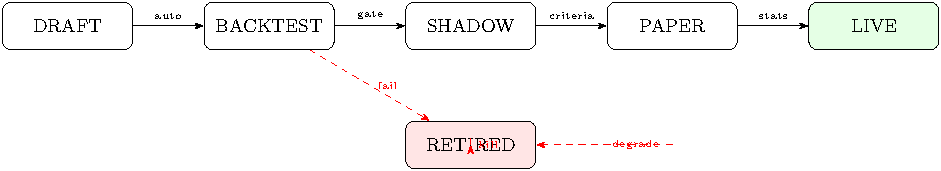
\includegraphics[width=0.95\textwidth]{figures/autonomy_pipeline.pdf}
    \caption{Experiment lifecycle pipeline with hard safety gates. DRAFT experiments transition through BACKTEST (historical validation), SHADOW (simulated bankroll), PAPER (statistical validation), and LIVE\_PROMOTED stages. Health-based kill checks (drawdown, Sharpe, Brier score) enforce automatic retirement for failed strategies.}
    \label{fig:autonomy_pipeline}
\end{figure}

The autonomy framework is not a proof of safety but an engineering discipline: every autonomous capability is wrapped in deterministic gates that are enforced in code, not merely documented in policy. As \citet{russell2020human} argues, truly beneficial AI requires not just intelligent behavior but also robust containment of that intelligence's side effects. Our bounded autonomy framework is a practical instantiation of that principle for financial systems.
